\section{Methods and Results}


\subsection{Pipeline Overview}

\begin{frame}
\frametitle{Pipeline Overview}
	\begin{columns}
		\begin{column}{0.5\textwidth}
			\begin{itemize}
				\uncover<1->{\item Starting point is HCP preprocessed data}
				\uncover<2->{\item Smoothing changed to 4mm}
				\uncover<3->{\item Singal-to-noise ratio increase, registrastion to MNI-152,\\enables statistical comparisons}
			\end{itemize}
		\end{column}

		\begin{column}{0.49\textwidth}
			\begin{itemize}
				\uncover<4->{\item Two analyses conducted (20s)}
				\uncover<5->{\item N-Back combination,\\4 copes/run,\\2 chunks/subject (2C),\\160 patterns total}
				\uncover<6->{\item N-Back distinction,\\8 copes/run,\\4 chunks/subject (4C),\\320 patterns total}
			\end{itemize}
		\end{column}
	\end{columns}	

	\begin{figure}
		\centering
		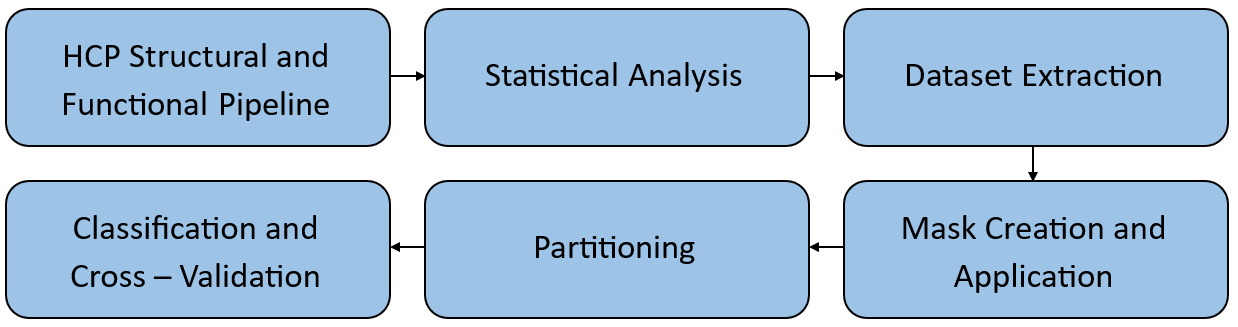
\includegraphics[width=0.98\textwidth]{assets/pipeline.png}
	\end{figure}
\end{frame}

\begin{frame}
\frametitle{Extraction and Masks}
	\begin{columns}
		\begin{column}{0.5\textwidth}
			\begin{itemize}
				\uncover<1->{\item From separate copes across different runs of various subjects into one dataset structure}
				\uncover<2->{\item Samples by Features matrix with attributes, targets, labels, chunks (\textbf{320 X 900k})}
			\end{itemize}
		\end{column}

		\begin{column}{0.49\textwidth}
			\begin{itemize}
				\uncover<3->{\item Two masks created\\for FFA and PPA\\with 12 voxel radius}
				\uncover<4->{\item Application of masks,\\focus on specific region,\\data is manageable\\(\textbf{320 X 1k})}
			\end{itemize}
		\end{column}
	\end{columns}

	\begin{figure}
		\centering
		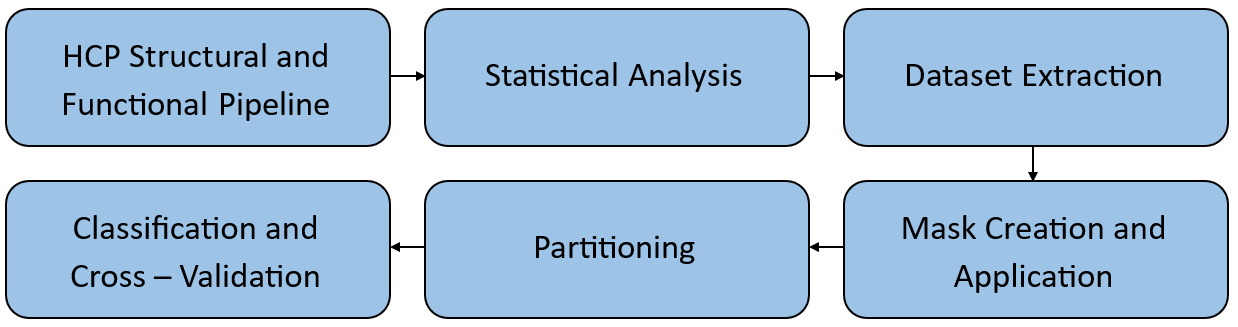
\includegraphics[width=0.98\textwidth]{assets/pipeline.png}
	\end{figure}
\end{frame}

\begin{frame}
\frametitle{Illustration of Masks}
	\begin{figure}
		\centering
		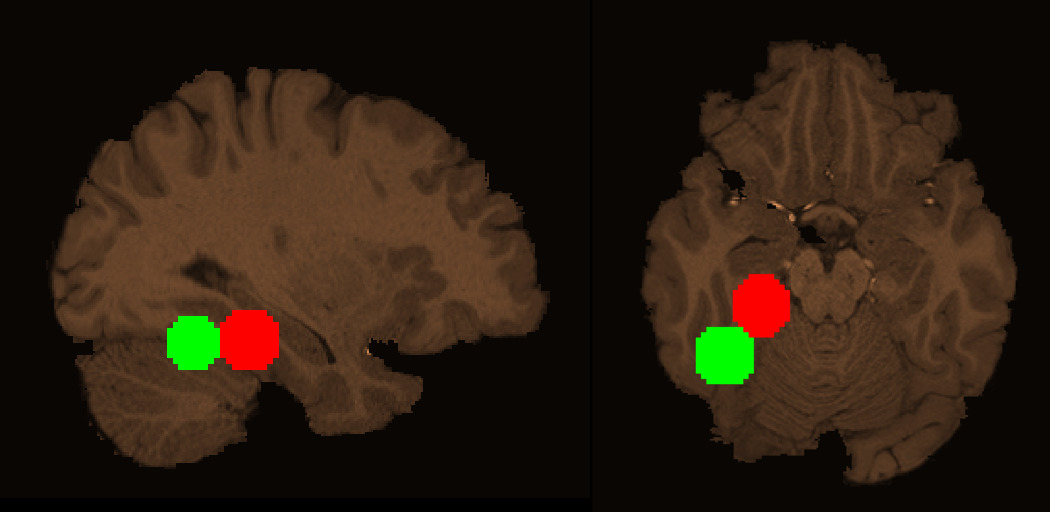
\includegraphics[width=0.98\textwidth]{assets/masks_sag_trans.jpg}
		\caption*{FSL Snapshots of FFA (green) and PPA (red) Masks at Maximum Overlap in the Saggital and Horizontal Planes}
	\end{figure}
\end{frame}

\begin{frame}
\frametitle{Partitioning, Classification and Cross-Validation}
		\begin{itemize}
			\uncover<1->{\item Partition data into folds, based on chunks}
			\uncover<2->{\item Each fold contains independent train and test sets (80/20)}
			\uncover<3->{\item SVM classification}
			\uncover<4->{\item Predict test set targets/labels}
			\uncover<5->{\item Repeat across multiple folds (cross-validate)}
		\end{itemize}

	\begin{figure}
		\centering
		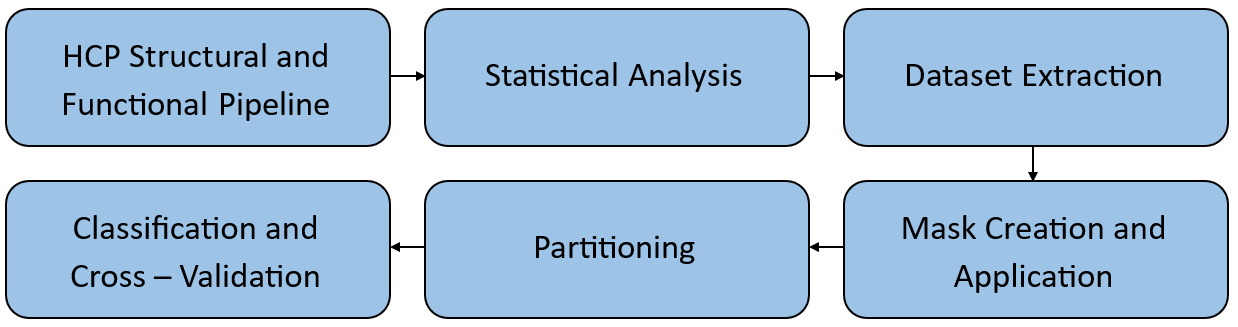
\includegraphics[width=0.98\textwidth]{assets/pipeline.png}
	\end{figure}
\end{frame}


\subsection{Data Analysis - UPA}

\begin{frame}
\frametitle{Category‐Secific BOLD Signal (\textit{UPA}) - PPA}
	\begin{columns}
		\begin{column}{0.5\textwidth}
			\begin{figure}
				\centering
				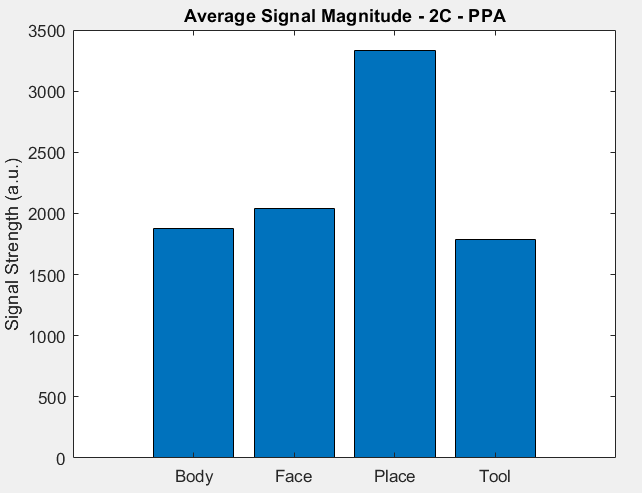
\includegraphics[width=0.98\textwidth]{assets/upa_2C_ppa.png}
			\end{figure}
		\end{column}

		\begin{column}{0.49\textwidth}
			\begin{figure}
				\centering
				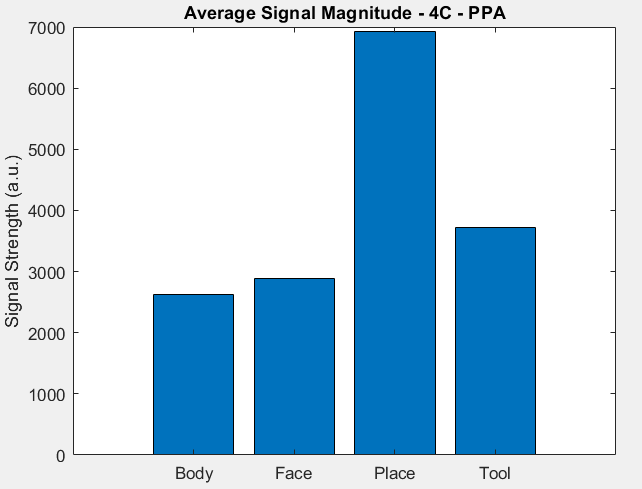
\includegraphics[width=0.98\textwidth]{assets/upa_4C_ppa.png}
			\end{figure}
		\end{column}
	\end{columns}	
	\begin{itemize}
		\item Average magnitude of brain activation in the PPA\\across different stimulus categories in the 2C and 4C analyses
		\item UPA based on COPE values -\\Statistical value of BOLD over time and voxels
		\item Baseline signal for the region's specificity stands out,\\with higher magnitude
	\end{itemize}
\end{frame}

%\begin{frame}
%\frametitle{Category‐Secific BOLD Signal (\textit{UPA}) - FFA}
%	\begin{columns}
%		\begin{column}{0.5\textwidth}
%			\begin{figure}
%				\centering
%				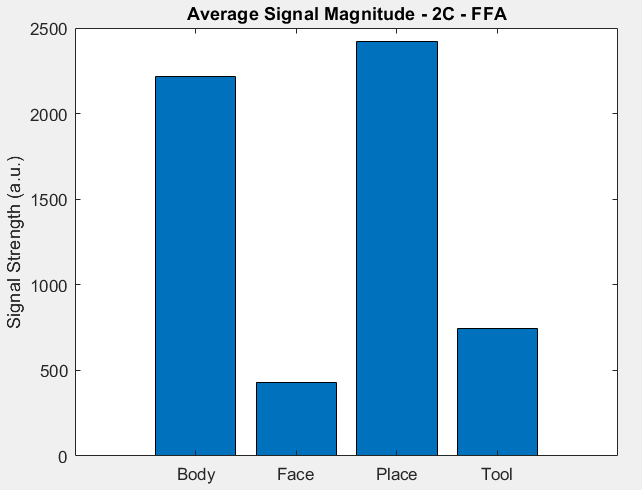
\includegraphics[width=0.98\textwidth]{assets/upa_2C_ffa.png}
%			\end{figure}
%		\end{column}
%
%		\begin{column}{0.49\textwidth}
%			\begin{figure}
%				\centering
%				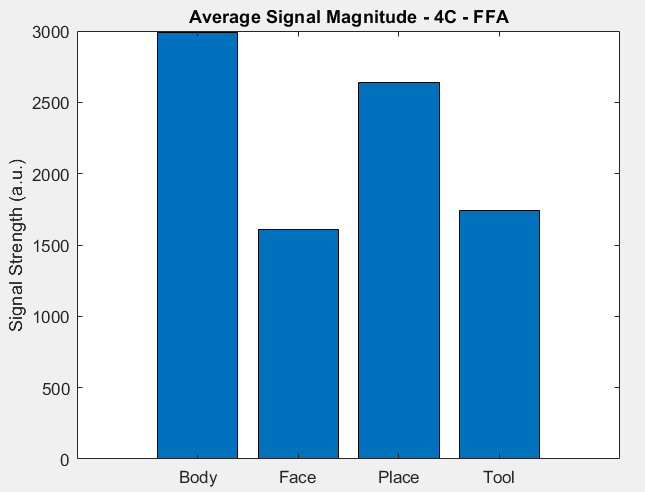
\includegraphics[width=0.98\textwidth]{assets/upa_4C_ffa.png}
%			\end{figure}
%		\end{column}
%	\end{columns}	
%	\begin{itemize}
%		\item Average magnitude of brain activation in the FFA\\across different stimulus categories in the 2C and 4C analyses
%		\item Irregularity: signal for faces is relatively weak
%		\item Baseline signal for the region's specificity still stands out,\\with lower magnitude
%	\end{itemize}
%\end{frame}

%\begin{frame}
%\frametitle{Central FFA - UPA}
%	\begin{columns}
%		\begin{column}{0.5\textwidth}		
%			\begin{itemize}
%				\uncover<1->{\item UPA repeated for the FFA\\using a 6 voxel radius mask}
%				\uncover<2->{\item Signal profile is canonical}
%				\uncover<3->{\item Residual signal in the outskirts, neighbouring with other areas}
%				\uncover<4->{\item Faces were presented after bodies and places, never after a fixation period}
%				\uncover<5->{\item MVPA efficacy uncompromised}
%			\end{itemize}
%		\end{column}
%
%		\begin{column}{0.49\textwidth}
%			\begin{figure}
%				\centering
%				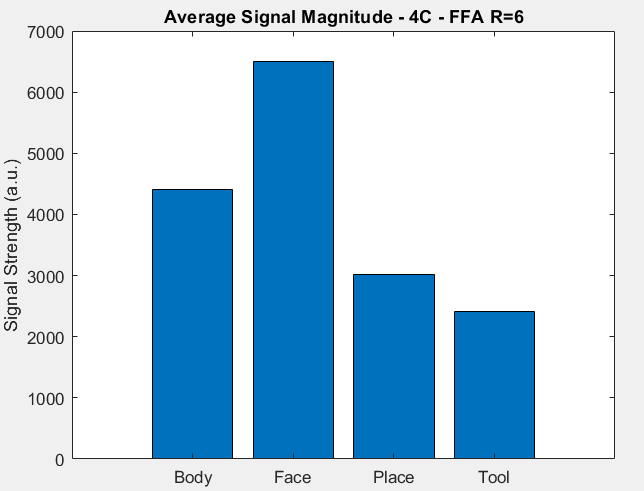
\includegraphics[width=0.98\textwidth]{assets/upa_4C_ffa_6.png}
%				\caption*{Average Magnitude of Brain Activation in the Central FFA}
%			\end{figure}
%		\end{column}
%	\end{columns}	
%\end{frame}

\begin{frame}
\frametitle{Classifier Performance Variables}
	\begin{columns}
		\begin{column}{0.5\textwidth}		
			\begin{itemize}
				\uncover<1->{\item Classification accuracy was treated as a function of\\three variables:}
				\uncover<2->{\item Chunks Per Subject}
				\uncover<3->{\item Fold Count}
				\uncover<4->{\item Subject Count}
			\end{itemize}
		\end{column}

		\begin{column}{0.49\textwidth}
			\begin{itemize}
				\uncover<5->{\item Outlier subjects were\\identified and excluded}
				\uncover<6->{\item Only subject with 0\% accuracy\\in both regions}
				\uncover<7->{\item Inability attributed to left FFA/PPA predominant activation or artifacts}
			\end{itemize}
		\end{column}
	\end{columns}	
\end{frame}


\subsection{Data Analysis - MVPA in the FFA}

\begin{frame}
\frametitle{MVPA - FFA - Chunks per Subject}

\centering
\makebox[0.5\textwidth]{\textbf{2C}}
\makebox[0.49\textwidth]{\textbf{4C}}

\vspace{0.2cm}

	\begin{columns}
		\begin{column}{0.49\textwidth}		
			\begin{itemize}
				\uncover<1->{\item Optimal mean accuracy of\\70\% across 3000 folds}
				\uncover<2->{\item Distribution \textbf{not normal}\\Lilliefors: $p = 10^{-4}$}
			\end{itemize}
		\end{column}

		\begin{column}{0.49\textwidth}
			\begin{itemize}
				\uncover<1->{\item Optimal mean accuracy of\\61.9\% across 3000 folds}
				\uncover<2->{\item Distribution \textbf{not normal}\\Lilliefors: $p = 10^{-4}$}
			\end{itemize}
		\end{column}
	\end{columns}

\vspace{0.2cm}

		\begin{itemize}
			\uncover<3->{\item Two-Sample F-Test showed different variances with $p < 10^{-16}$}
			\uncover<4->{\item Wilcoxon Rank-Sum Test showed:\\statistically significant difference in distribution means with $p < 1^{-16}$}
		\end{itemize}
\end{frame}

\begin{frame}
\frametitle{MVPA - FFA - Chunks per Subject - Conclusions}
	\begin{itemize}
			\uncover<1->{\item The different methods of integrating separate N-Back data provide significantly different results}
			\uncover<2->{\item The tool should preferentially be trained and utilized on\\data belonging to only one N-Back paradigm}
			\uncover<3->{\item Supervised learning data should come from a study separating\\N-Back paradigms, in different sessions, not just blocks or trials}
			\uncover<4->{\item If a generic approach is unavoidable, efficiency prevails}
	\end{itemize}
\end{frame}


\begin{frame}
\frametitle{MVPA - FFA - Fold Count}
	\begin{itemize}
		\uncover<1->{\item Data from 19 subjects classified across 250:250:3000 folds}
		\uncover<2->{\item Accuracy stabilized to 2nd decimal by 250 folds\\
					    with $\sigma = 0.15\%$ and $\sigma = 0.17\%$\\for analysis 2C and 4C, respectively}
		\uncover<3->{\item Slight overperformance until 1000 folds}
		\uncover<4->{\item Practical fold count was determined for each analysis}
	\end{itemize}
\end{frame}

\begin{frame}
\frametitle{MVPA - FFA - 3000 Folds Analysis}
	\begin{columns}
		\begin{column}{0.49\textwidth}		
			\begin{itemize}
				\uncover<1->{\item Mean: 70\%\hspace{0.8cm}$\sigma$: 8.4\%\\
							    Median: 71.4\%}
			\end{itemize}
			\begin{figure}
				\centering
				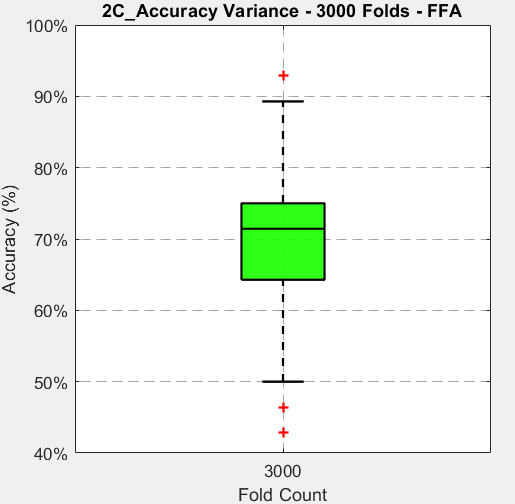
\includegraphics[width=0.98\textwidth]{assets/box_2C_3000_ffa.png}
			\end{figure}
		\end{column}

		\begin{column}{0.49\textwidth}
			\begin{itemize}
				\uncover<1->{\item Mean: 61.9\%\hspace{0.8cm}$\sigma$: 6.3\%\\
							    Median: 62.5\% }
			\end{itemize}
			\begin{figure}
				\centering
				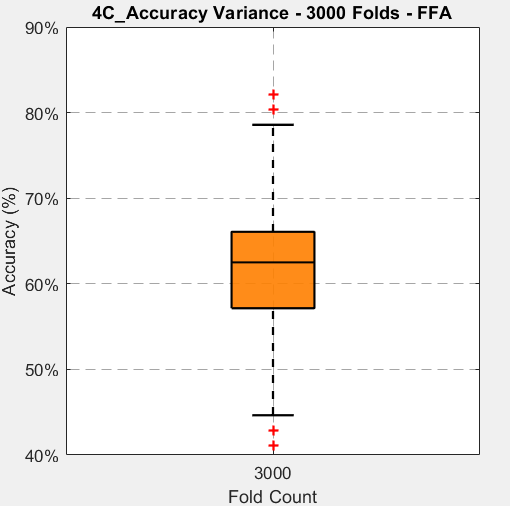
\includegraphics[width=0.98\textwidth]{assets/box_4C_3000_ffa.png}
			\end{figure}
		\end{column}
	\end{columns}
\end{frame}


\begin{frame}
\frametitle{MVPA - FFA - Practical Fold Count}
	\begin{columns}
		\begin{column}{0.49\textwidth}		
			\begin{itemize}
				\uncover<1->{\item Mean: 72.3\%\hspace{0.8cm}$\sigma$: 8.0\%\\
						   	    Median: 71.4\%}
			\end{itemize}
			\begin{figure}
				\centering
				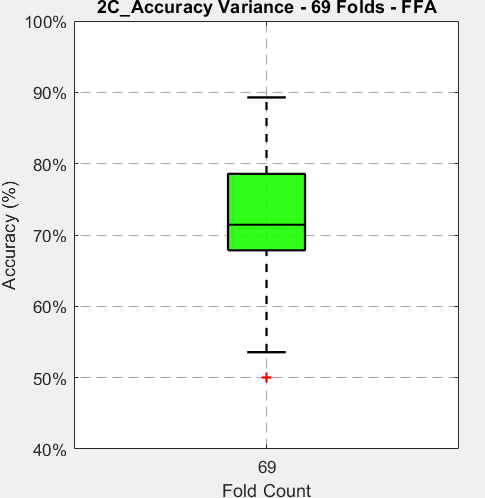
\includegraphics[width=0.98\textwidth]{assets/box_2C_69_ffa.png}
			\end{figure}
		\end{column}

		\begin{column}{0.49\textwidth}
			\begin{itemize}
				\uncover<1->{\item Mean: 62.2\%\hspace{0.8cm}$\sigma$: 6.0\%\\
							    Median: 62.5\%}
			\end{itemize}
			\begin{figure}
				\centering
				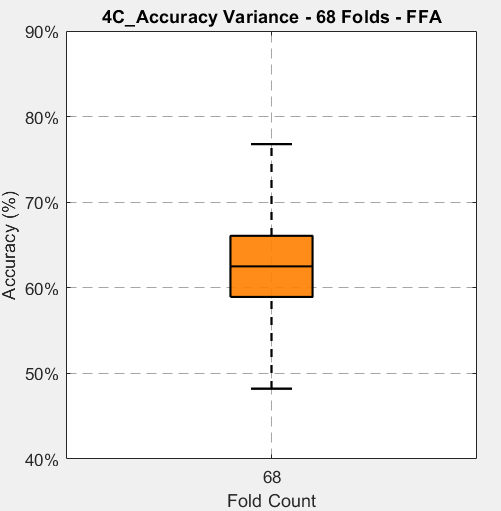
\includegraphics[width=0.98\textwidth]{assets/box_4C_68_ffa.png}
			\end{figure}
		\end{column}
	\end{columns}
\end{frame}

\begin{frame}
\frametitle{MVPA - FFA - 2C Subject Count}
	\begin{figure}
		\centering
		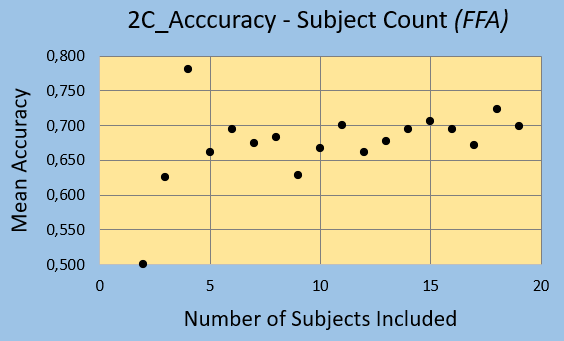
\includegraphics[width=0.98\textwidth, height=5cm]{assets/subj_count_2C_ffa.png}
	\end{figure}

	\begin{itemize}
		\uncover<1->{\item Surprisingly accurate at 2 subjects only (50\%)}
		\uncover<2->{\item Irregularity at 4 subjects (78.1\%), affected by low fold counts}
		\uncover<3->{\item Realistic values over 6 subjects}
		\uncover<4->{\item Oscillates in the 65-70\% range thereafter}
	\end{itemize}
\end{frame}

\begin{frame}
\frametitle{MVPA - FFA -  4C Subject Count}
	\begin{figure}
		\centering
		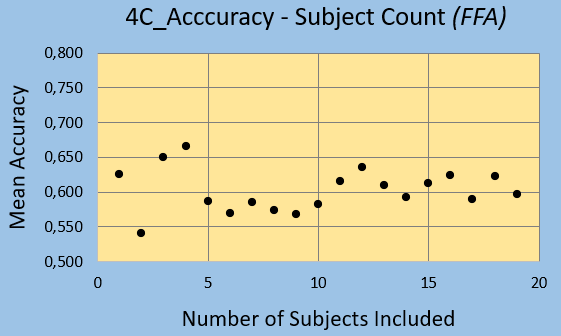
\includegraphics[width=0.98\textwidth, height=5cm]{assets/subj_count_4C_ffa.png}
	\end{figure}

	\begin{itemize}
		\uncover<1->{\item Similar overperformance before 5 subjects}
		\uncover<2->{\item Stabilizes around 57\% initially at 5 subjects}
		\uncover<3->{\item Realistic values over 11 subjects}
	\end{itemize}
\end{frame}

\subsection{Data Analysis - MVPA in the PPA}

\begin{frame}
\frametitle{MVPA - PPA - Chunks per Subject}

\centering
\makebox[0.5\textwidth]{\textbf{2C}}
\makebox[0.49\textwidth]{\textbf{4C}}

\vspace{0.2cm}

	\begin{columns}
		\begin{column}{0.49\textwidth}		
			\begin{itemize}
				\uncover<1->{\item Optimal mean accuracy of\\66.4\% across 3000 folds}
				\uncover<2->{\item Distribution \textbf{not normal}\\Lilliefors: $p = 10^{-4}$}
			\end{itemize}
		\end{column}

		\begin{column}{0.49\textwidth}
			\begin{itemize}
				\uncover<1->{\item Optimal mean accuracy of\\50.6\% across 3000 folds}
				\uncover<2->{\item Distribution \textbf{not normal}\\Lilliefors: $p = 10^{-4}$}
			\end{itemize}
		\end{column}
	\end{columns}

\vspace{0.2cm}

		\begin{itemize}
			\uncover<3->{\item Two-Sample F-Test showed different variances with $p < 10^{-16}$}
			\uncover<4->{\item Wilcoxon Rank-Sum Test showed:\\statistically significant difference in distribution means with $p < 1^{-16}$}
			\vspace{0.2cm}
			\uncover<5->{\item Choice of data integration shows identical pattern in both brain regions}
		\end{itemize}
\end{frame}

\begin{frame}
\frametitle{MVPA - PPA - Fold Count}
	\begin{itemize}
		\uncover<1->{\item Data from 19 subjects classified across 250:250:3000 folds}
		\uncover<2->{\item Accuracy stabilized to 2nd decimal by 250 folds\\
					    with $\sigma = 0.12\%$ and $\sigma = 0.07\%$}
		\uncover<3->{\item Slight underperformance until 750 folds}
		\uncover<4->{\item Absolute stability by 750 folds (third decimal)\\
					    Improvement might be due to signal baseline}
		\uncover<5->{\item Practical fold count was determined for each analysis}
	\end{itemize}
\end{frame}

\begin{frame}
\frametitle{MVPA - PPA - 3000 Folds}
	\begin{columns}
		\begin{column}{0.49\textwidth}		
			\begin{itemize}
				\uncover<1->{\item Mean: 66.4\%\hspace{0.8cm}$\sigma$: 7.9\%\\
							    Median: 65.6\%}
			\end{itemize}
			\begin{figure}
				\centering
				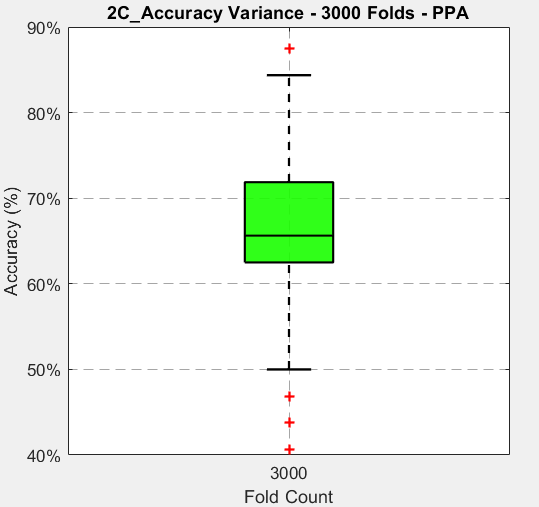
\includegraphics[width=0.98\textwidth]{assets/box_2C_3000_ppa.png}
			\end{figure}
		\end{column}

		\begin{column}{0.49\textwidth}
			\begin{itemize}
				\uncover<1->{\item Mean: 50.6\%\hspace{0.8cm}$\sigma$: 6.1\%\\
							    Median: 50.0\%}
			\end{itemize}
			\begin{figure}
				\centering
				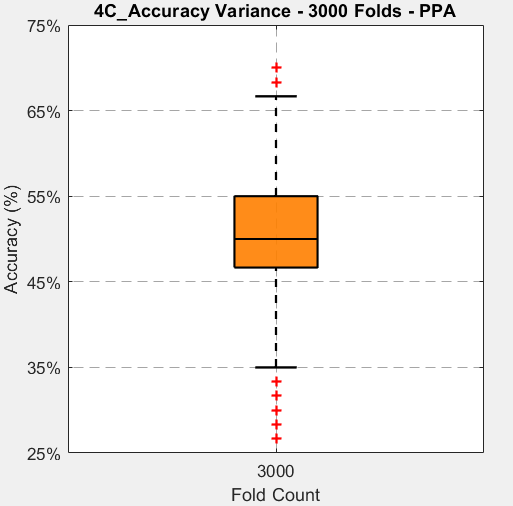
\includegraphics[width=0.98\textwidth]{assets/box_4C_3000_ppa.png}
			\end{figure}
		\end{column}
	\end{columns}
\end{frame}


\begin{frame}
\frametitle{MVPA - PPA - Practical Fold Count}
	\begin{columns}
		\begin{column}{0.49\textwidth}		
			\begin{itemize}
				\uncover<1->{\item Mean: 66.4\%\hspace{0.8cm}$\sigma$: 7.0\%\\
							    Median: 65.6\%}
			\end{itemize}
			\begin{figure}
				\centering
				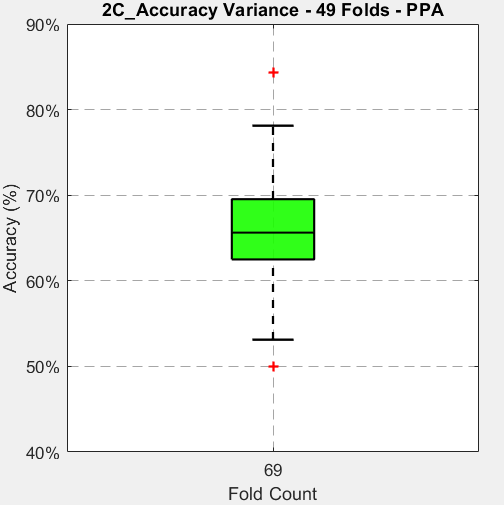
\includegraphics[width=0.98\textwidth]{assets/box_2C_49_ppa.png}
			\end{figure}
		\end{column}

		\begin{column}{0.49\textwidth}
			\begin{itemize}
				\uncover<1->{\item Mean: 50.1\%\hspace{0.8cm}$\sigma$: 5.7\%\\
							    Median: 50.0\%}
			\end{itemize}
			\begin{figure}
				\centering
				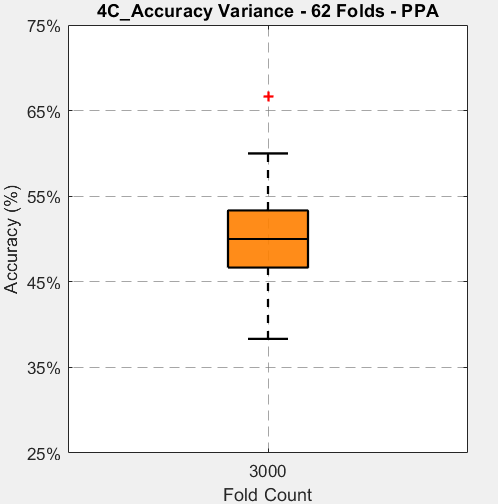
\includegraphics[width=0.98\textwidth]{assets/box_4C_62_ppa.png}
			\end{figure}
		\end{column}
	\end{columns}
\end{frame}


\begin{frame}
\frametitle{MVPA - PPA -  2C Subject Count}
	\begin{figure}
		\centering
		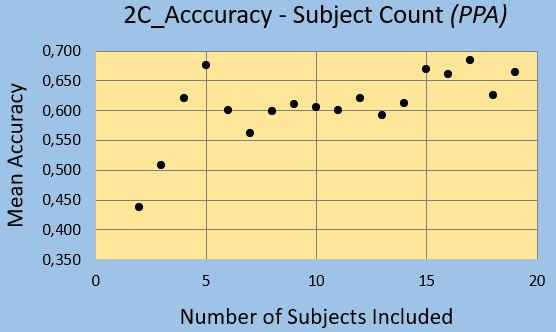
\includegraphics[width=0.98\textwidth, height=5cm]{assets/subj_count_2C_ppa.png}
	\end{figure}

	\begin{itemize}
		\uncover<1->{\item Rapid linear increase until 5 subjects}
		\uncover<2->{\item Overperformance at 5 (67.5\%), cannot be generalized}
		\uncover<3->{\item Consistency over 5 subjects around 60\%}
		\uncover<4->{\item Approaches optimal accuracy at 15 subjects (66.8\% - 66.4\%)}
	\end{itemize}
\end{frame}

\begin{frame}
\frametitle{MVPA - PPA -  4C Subject Count}
	\begin{figure}
		\centering
		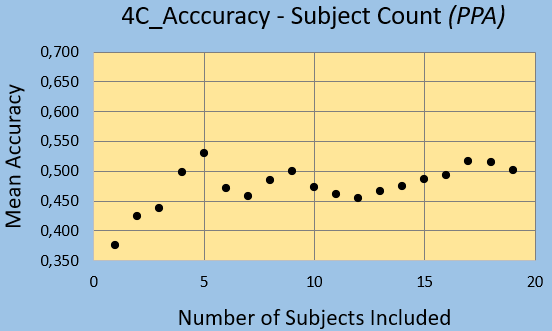
\includegraphics[width=0.98\textwidth, height=5cm]{assets/subj_count_4C_ppa.png}
	\end{figure}

	\begin{itemize}
		\uncover<1->{\item Similar pattern showing even more stability}
		\uncover<2->{\item Linear increase into irregularity at 5}
		\uncover<3->{\item Oscillation around optimal accuracy (50.1\%)}
	\end{itemize}
\end{frame}

\begin{frame}
\frametitle{Summary}
	\begin{itemize}
		\uncover<1->{\item Automated and provided protocol for data cleanup and selection}
		\uncover<2->{\item Automated data extraction and consolidation}
		\uncover<3->{\item Linked base signal to performance}
		\uncover<4->{\item Significance of reasearcher's choice of data interpretation proven}
		\uncover<5->{\item Provided framework for tool's optimal performance, efficiency, practicality}
	\end{itemize}
\end{frame}

\begin{frame}
\frametitle{Future Work}
	\begin{itemize}
		\uncover<1->{\item Script optimization, grouping and potetntially GUI}
		\uncover<2->{\item Cross-model decoding}
		\uncover<3->{\item Utilization of more specialized data}
		\uncover<4->{\item Expansion to other brain regions, not only visual}
		\uncover<5->{\item Big Picture, Clinical Applications, Diagnosis, Cure}
		\uncover<6->{\item Bigger Picture, Brain-Computer Interface}
	\end{itemize}
\end{frame}